\vspace{-3mm}
\section{Method}
% \noindent\textbf{Entropy and Mutual Information.}
% For a random variable $X$, entropy is $H(X\mid c) = -\sum_x p(x\mid c) \log p(x)$. 
% For multiple variables, joint entropy satisfies:
% \begin{equation}
% H(X_1,\dots,X_n) \le \sum_{i=1}^n H(X_i).
% \end{equation}
% We use $H^{(\ell)}(z_t)$ to denote entropy of the predicted categorical distribution of $\ell$-th token by model under state $z_t$.

% The mutual information between variables $\{X_i\}$ and $Y$ is bounded by:
% \begin{equation}
% I(\{X_i\}; Y) \le \min\left\{H(Y), \ \sum_{i=1}^n H(X_i)\right\}.
% \end{equation}

\subsection{Motivation}
\label{sec:motivation}
Existing certainty-based sampling methods typically employ a greedy strategy. These methods aim to minimize error accumulation by prioritizing the most certain positions. While this approach effectively reduces immediate uncertainty and enhances short-term reliability, it essentially performs a greedy optimization of the cumulative uncertainty. This leads us to a fundamental question:

\begin{observationbox}
\textbf{Question 1:}
Is greedy optimization closed to minimize cumulative uncertainty across steps?
\end{observationbox}

To quantify the uncertainty throughout a generation process $\tau =z_T\rightarrow z_{T-1}\rightarrow\ldots\rightarrow z_0$ , we first introduce 
\textbf{Cumulative Entropy} $\tilde{H}$ over $\tau$ as a key metric, defined as:
\begin{equation}
    \tilde{H}(\tau):= \sum_{t=T}^{1} C(a_t \mid z_t),
\end{equation}
where $C(a_t\mid z_t) = \sum_{\ell \in A_t} H^{(\ell)}(z_t)$ represents the sum of marginal entropy for the tokens selected at step $t$, given by the model's output distribution. This metric quantifies the total uncertainty accumulated throughout the decoding trajectory.

To explore this question, we present two case studies that illustrate the limitations of greedy samplers.

\noindent \textbf{Case Study 1: One-way Multiplication.}  
The model is tasked with generating an equation \(a \times b = c\), where \(a\) and \(b\) are decimal factors and \(c\) is a binary product. This task is {inherently one-way}: computing a product from factors is straightforward, while factoring is not only computationally difficult but also particularly challenging for MDMs to generate, especially when the product is represented in binary format. Two decoding paths emerge: (i) \textit{Product-first}, and (ii) \textit{Factor-first}. 

A greedy sampler mistakenly favors path (i) because the binary digits of \(c\) exhibit lower per-token uncertainty (requiring a choice only from \(\{0,1\}\)) than the decimal digits of \(a\) and \(b\) (which have 10 possible values). As shown in Figure~\ref{fig:toy_analysis}, by minimizing immediate uncertainty, the greedy strategy commits to a product without fixing the factors, leading to incorrect equations and high residual uncertainty. Conversely, an optimal strategy would resolve the higher-uncertainty factors \(a\) and \(b\) first; once fixed, \(c\) can be determined with nearly zero uncertainty. Empirically, the greedy certainty-based sampler (represented by Entropy~\cite{ye2025dream}) prioritizes path (i) with 73.2\% probability, leading to significantly higher cumulative uncertainty.

\noindent \textbf{Case Study 2 : Binary Judgment.}
In this experiment, the model is tasked with judging the truth of an arithmetic statement using the template: ``[reasoning-masks] The answer is (Yes/No): [answer-mask]''. The answer token typically exhibits lower local uncertainty as it is constrained to a binary choice (Yes/No), whereas the reasoning steps involve much higher uncertainty. Consequently, greedy samplers tend to decode the answer token prematurely, making a commitment before the underlying reasoning is resolved. This leads to incorrect judgments and leaves high residual uncertainty in the reasoning positions. 

To analyze this, we compare greedy certainty-based samplers against an auto-regressive (AR) baseline, which naturally resolves high-uncertainty reasoning before the binary answer. As shown in Table~\ref{tab:toy_experiment_2}, the AR baseline achieves superior accuracy and lower cumulative uncertainty, highlighting that greedy MDM samplers fail by prematurely committing to low-uncertainty answer tokens before the reasoning is established. 
\begin{table}[h]
\centering
\caption{Quantitative results for Case Study 2.}
\label{tab:toy_experiment_2}
\small
\setlength{\tabcolsep}{3pt}
\begin{tabular}{@{}lccccc@{}}
\toprule
\textbf{Metric} & {Entropy} & {Confidence} & {Margin} & {AR} \\ \midrule
$\tilde{H}$ $\downarrow$ & 32.75 & 31.68 & 35.60 & \textbf{25.19} \\
Acc. (\%) $\uparrow$ & 67 & 73 & 66 & \textbf{90} \\ \bottomrule
\end{tabular}
\end{table}

\begin{observationbox}
\textbf{Observation 1:}\label{obs:obs1}
Existing greedy certainty-based samplers often fail to find near-optimal decoding paths.
\end{observationbox}

As illustrated in Figure~\ref{fig:toy_analysis}, an optimal decoding action should be evaluated not only by its own prediction certainty but also by the \textit{information gain} it provides for the remainder of the generation process. To address the limitations of existing samplers, it is essential to account for this information gain when making current decisions. As shown in Figure~\ref{fig:toy_analysis}, our proposed Info-Gain Sampler effectively addresses this one-way challenge by prioritizing the decoding of factors with an 84\% probability.

In standard ARMs, assessing information gain typically requires computationally expensive techniques, such as Monte Carlo Tree Search, to simulate future trajectories. This is primarily due to the next-token bottleneck: since ARMs only provide the probability of the immediate next token, multi-step look-ahead becomes prohibitively slow.

\begin{observationbox}
\textbf{Question 2:}
Can Masked Diffusion Models efficiently assess information gain of a decoding action?
\end{observationbox}


Unlike ARMs, MDMs don't have the next-token bottleneck. MDMs leverage bidirectional attention, allowing the model to simultaneously evaluate the impact of any decoding action on the uncertainty of the entire sequence. This architectural advantage enables the model to “see” how filling a mask affects the uncertainty of all remaining masks in a single forward pass.

\begin{observationbox}
\textbf{Observation 2:}\label{obs:obs2} MDMs' bidirectional architecture enables efficient information gain estimation in one forward pass, bypassing expensive iterative computations.
\end{observationbox}

\subsection{Information Gain Sampler}  

\label{sec:method_info_gain}
The insights from \textbf{Observation 1} and \textbf{Observation 2} suggest that greedy optimization alone is insufficient for minimizing cumulative uncertainty across the entire sequence. 

We introduce the \textbf{Information Gain (Info-Gain) Sampler} which leverages the bidirectional nature of MDMs to balance the immediate uncertainty cost of a decoding decision against its expected information gain over the remaining masked positions.

\subsubsection{Objective of Info-Gain Sampler}
We first define \textbf{state uncertainty} as the average marginal entropy over the masked positions in state $z_t$:
\begin{equation}
\mathcal{H}(z_t)=\frac{1}{|\mathcal{M}_{t}|} \sum_{\ell \in \mathcal{M}_{t}} H^{(\ell)}(z_t)
\end{equation}
The state uncertainty quantifies the information remaining to be resolved by the model and can be computed efficiently via a single forward pass. 
%For a fully decoded sequence, the state uncertainty is defined as zero.

The \textbf{information gain} of action $a_t$ is defined as the reduction in state uncertainty (equivalently, the decrease in marginal entropy over the remaining masked positions) it induces:
\begin{equation}
    \text{IG}(a_t ; z_t) := \mathcal{H}(z_t) - \mathcal{H}(z_{t-1})
\end{equation}
where $z_{t-1} = \text{Apply}(z_t, a_t)$ denotes the state obtained after executing action $a_t$ from state $z_t$.

The total impact of a decoding action $a_t$ is thus decomposed into two components:

\textbf{(1) Immediate Cost:} the uncertainty of the tokens being decoded in the current step, measured by the sum of marginal entropy over the chosen positions $C(a_t \mid z_t)$.

\textbf{(2) Information Gain:} the reduction in the uncertainty over the remaining mask positions, quantified by the information gain $\text{IG}(a_t; z_t)$.

To balance these two components, we define the Info-Gain Sampler objective as:
\begin{equation}
J_{IG}(a_t \mid z_t) = \underbrace{\text{IG}(a_t ;z_t)}_{\text{Information Gain}}-\underbrace{C(a_t \mid z_t)}_{\text{Immediate Cost}},
\label{eq:igp_objective}
\end{equation}

We provide further theoretical analysis in Appendix~\ref{appendix:mi_upper_bound}.

\subsubsection{Implementation of Info-Gain Sampler}
\begin{figure}[t]
    \centering
    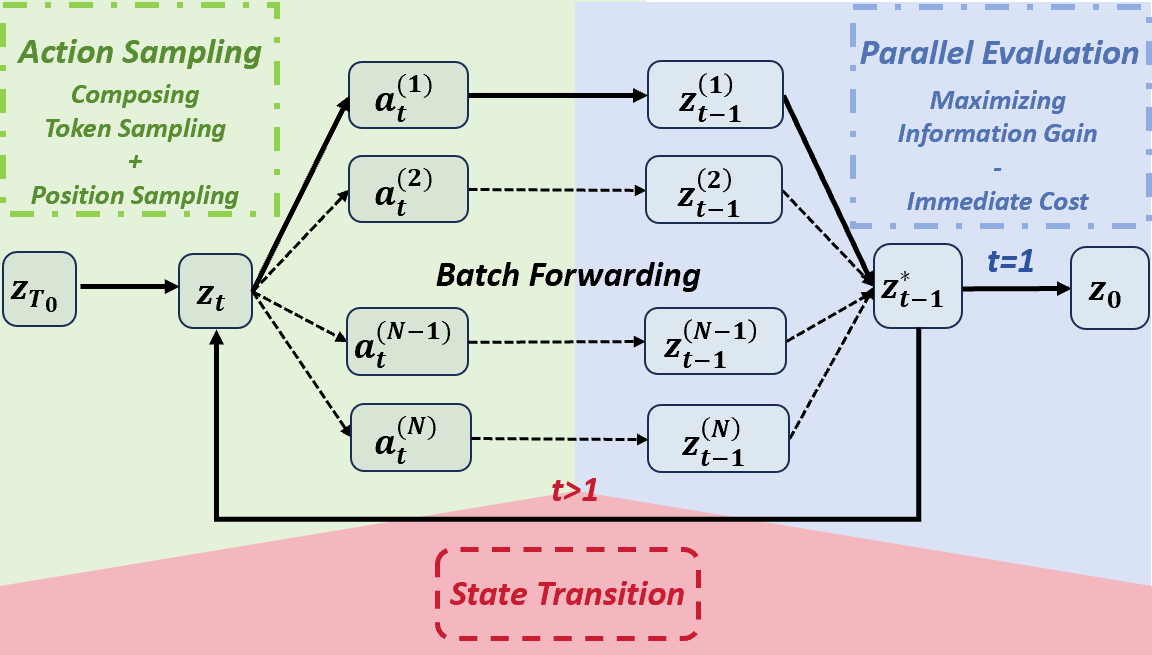
\includegraphics[width=1\linewidth]{workflow_v2.png}
    \caption{The Info-Gain Sampler workflow. Starting from state $z_{T_0}$, the sampler iteratively: (1) samples candidate actions, (2) evaluates $J_{\text{IG}} = \text{Immediate Cost} - \text{Information Gain}$ in parallel to select the optimal successor state $z_{t-1}^*$, and (3) executes the state transition until reaching the final sequence $z_0$.}
    \label{igp_workflow}
\end{figure}


\noindent\textbf{Action Sampler.} Following previous work~\cite{opendllm2025,yang2025mmada}, we explore the large action space by generating a candidate set $\mathcal{C}$ of size $N$ through a two-stage sampling process: (1) \textit{Token Sampling}: drawing tokens $v_\ell$ from $p_\theta$ with token temperature $\tau_{\text{token}}$, and (2) \textit{Position Sampling}: selecting positions $\ell \in \mathcal{M}_t$ using a softmax over certainty scores $\phi(\ell,z_t)$ with position temperature $\tau_{\text{pos}}$. Each candidate action $a_t = \{(\ell, v_\ell)\}$ is formed by pairing these samples, providing a diverse and high-quality set for evaluation. The size of $a_t$ is determined by a step scheduling function.


At each decoding step, Info-Gain Sampler follows a three-step cycle to determine and execute the most informative action (Figure~\ref{igp_workflow}):

\textbf{(1) Sampling:} We sample a candidate set $\mathcal{C} = \{a_t^{(1)}, \dots, a_t^{(N)}\}$ of diverse actions using the \textit{Action Sampler}. This step explores the combinatorially large action space by proposing multiple potential actions.

\textbf{(2) Evaluation:} We compute the objective $J(a_t\mid z_t)$ for all candidates $a_t$ in the set $\mathcal{C}$. Crucially, as noted in the previous section, this evaluation is highly efficient as it requires only a single batched forward pass to estimate the future information gain for all candidates simultaneously.

\textbf{(3) Transition:} The optimal action is selected as $a_t^* = \arg\max_{a\in \mathcal{C}} J_{IG}(a \mid z_t)$. We then execute this action to transition to the next state $z_{t-1}^*$, repeating the cycle until all masked positions are filled and a complete sequence is generated.


\subsubsection{Efficient Implementation of Info-Gain Sampler}
\label{sec:acceleration}
To ensure efficiency, candidate evaluations are performed in parallel within a single batched forward pass. We further optimize the sampler by restricting the information-gain computation to the current active block $\mathcal{B}$~\citep{arriola2025block}, which enables effective KV caching. Additionally, we implement a high-confidence bypass: if the maximum token probability exceeds a threshold $\gamma$, the corresponding positions are directly fixed into the action set. If the number of such high-confidence positions exceeds the predefined size of the action set for the current step, only the top-$k$ positions with the highest confidence are selected for decoding. This hybrid approach, inspired by \citet{wu2025fast}, significantly reduces inference latency while preserving planning quality. Because Info-Gain effectively reduces uncertainty during decoding, the high-confidence bypass is triggered more frequently, making the mechanism exceptionally efficient.


\subsubsection{Why is Info-Gain effective}

\textbf{State uncertainty} serves as an effective indicator for determining whether the current decoding state lies close to the \textbf{training data manifold}. When the decoded content is logically coherent and fluently expressed, the state resides near the data manifold, resulting in a concentrated predictive probability distribution and low uncertainty. Conversely, if the model lacks sufficient training on certain text forms, once decoding enters such inadequately covered regions during inference, it exhibits characteristics of a dispersed probability distribution and high uncertainty. Since the training data distribution represents logically sound and semantically coherent text forms, high uncertainty suggests that the current state may have deviated from the data manifold, indicating potential logical errors or peculiar expressions.

Existing greedy certainty-based samplers share a fundamental limitation: they cannot recognize the data manifold deviation signals reflected by state uncertainty. These methods select the most certain action at each step, but locally certain actions do not necessarily correspond to actions that keep subsequent states on the data manifold. Local confidence cannot effectively determine whether an action will lead to future deviations. In contrast, the Info-Gain Sampler actively perceives and utilizes state uncertainty through its information-gain term. When a candidate action would cause the state to deviate from the data manifold, the resulting state exhibits increased uncertainty, which negatively impacts the information-gain term and prevents such actions from being prioritized. This mechanism of identifying and maintaining the data manifold through state uncertainty perception enables the Info-Gain Sampler to preserve logical coherence and fluent expression throughout the decoding path, even under high sampling temperatures.

\begin{table*}[!ht]
\centering
\caption{Performance on the full-attention MDM (\textbf{Dream-7B}). Results are reported with decoding rates $K \in \{1, 2\}$, where reasoning tasks(GSM8K, MATH500, HumanEval, MBPP) use a block size of 16 and planning tasks (Sudoku, Countdown) are decoded globally. We report the accuracy for each task, along with the average accuracy (Avg.) and cumulative entropy ($\tilde{H}$) per generation.}
\label{tab:dream_results}
\resizebox{\textwidth}{!}{
\begin{tabular}{llcccccccc}
\toprule
\textbf{K} & \textbf{Sampler} & \textbf{GSM8K} & \textbf{MATH500} & \textbf{HumanEval} & \textbf{MBPP} & \textbf{Sudoku} & \textbf{Countdown} &\textbf{Avg.}& \textbf{$\tilde{H}\downarrow$} \\
\midrule
\multirow{8}{*}{\makecell[l]{$2$}} 
  & Uniform & 18.7 & 14.3 & 14.3 & 18.6 & 52.8 & 7.6& 21.1 & 389.2 \\
  & Entropy & 55.8 & 27.0 & 26.2 & 23.2 & 76.0 & 23.2& 38.6 & 247.8 \\
& Confidence & 61.9 & 29.4 & 26.8 & 25.2 & 81.6& 36.2& 43.5 & 249.2 \\
& Margin & 65.5 & 28.8 & 28.8 & 23.6 & 74.4& 28.9& 41.7 & 287.5 \\
& KLASS & 67.3 & 30.4 & 31.9 & 30.1 & 82.1& 35.4& 46.2 & 239.3 \\
& PC-Sampler& 72.8 & 32.3 & 36.4 & 34.4 & 80.2& 42.4& 49.8 & 158.3 \\
& LookUM& 75.2 & 35.2 & 38.4 & 36.1 & 77.4 & 39.2 & 50.3 & 134.9 \\
& \textbf{Info-Gain} & \textbf{77.7} & \textbf{34.2} & \textbf{42.9} & \textbf{39.4} & \textbf{82.2} & \textbf{44.1} & \textbf{53.4} & \textbf{104.3} \\
\hdashline
\multirow{8}{*}{\makecell[l]{$1$}} 
  & Uniform & 30.4 & 15.8 & 16.7 & 30.8 & 60.4 & 8.8& 27.2 & 199.3 \\
  & Entropy & 75.7 & 47.0 & 46.4 & 45.0 & 78.8 & 33.6& 54.4 & 95.6 \\
& Confidence & 78.8 & 46.6 & 49.4 & 39.8 & 81.5 & 39.2& 55.9 & 99.5 \\
& Margin & 77.5 & 46.5 & 41.5 & 40.4 & 80.3 & 35.2& 53.6 & 107.3 \\
& KLASS & 78.2 & 47.2 & 34.2 & 40.6 & 79.9 & 34.3& 52.4 & 99.6 \\
& PC-Sampler& 81.5 & 46.8 & 54.4 & 46.2 & 83.6 & 41.8& 59.1 & 78.4 \\
& LookUM & 78.3 & 51.4 & 52.3 & 45.9 & 78.4 & 43.3 & 58.2 & 61.4 \\
& \textbf{Info-Gain} & \textbf{83.3} & \textbf{51.3} & \textbf{59.2} & \textbf{48.4} & \textbf{84.4}& \textbf{45.2} & \textbf{62.0} & \textbf{48.6} \\
\bottomrule
\end{tabular}
}
\vspace{-3mm}
\end{table*}